\documentclass[tikz,border=2pt]{standalone}
\usepackage{times}
\usepackage{amsmath,amssymb}
\usetikzlibrary{positioning,arrows.meta,fit,backgrounds}
\begin{document}
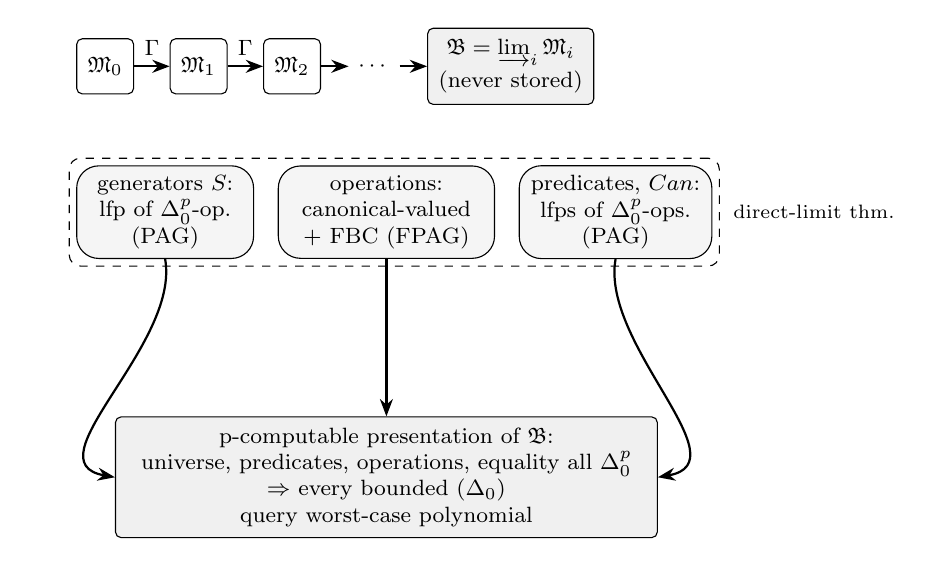
\begin{tikzpicture}[
  font=\footnotesize,
  box/.style={draw, rounded corners=2pt, align=center, inner sep=4pt, minimum height=7mm},
  pill/.style={draw, rounded corners=8pt, align=center, inner sep=3.5pt, fill=gray!8},
  arr/.style={-{Stealth[length=2.2mm]}, thick}
]
\node[box] (m0) {$\mathfrak{M}_0$};
\node[box, right=4.5mm of m0] (m1) {$\mathfrak{M}_1$};
\node[box, right=4.5mm of m1] (m2) {$\mathfrak{M}_2$};
\node[right=3.5mm of m2] (dots) {$\cdots$};
\node[box, right=3.5mm of dots, fill=gray!12, align=center] (lim) {$\mathfrak{B}=\varinjlim_i \mathfrak{M}_i$\\[1pt] (never stored)};
\draw[arr] (m0) -- node[above]{$\Gamma$} (m1);
\draw[arr] (m1) -- node[above]{$\Gamma$} (m2);
\draw[arr] (m2) -- (dots);
\draw[arr] (dots) -- (lim);
\node[pill, below=9mm of m0.south west, anchor=north west, text width=20mm] (p1) {generators $S$:\\ lfp of $\Delta^p_0$-op.\\ (PAG)};
\node[pill, right=3mm of p1, text width=25mm] (p2) {operations:\\ canonical-valued\\ $+$ FBC (FPAG)};
\node[pill, right=3mm of p2, text width=22mm] (p3) {predicates, $Can$:\\ lfps of $\Delta^p_0$-ops.\\ (PAG)};
\node[box, below=20mm of p2, fill=gray!12, text width=66mm, align=center] (out) {p-computable presentation of $\mathfrak{B}$:\\ universe, predicates, operations, equality all $\Delta^p_0$\\ $\Rightarrow$ every bounded ($\Delta_0$) query worst-case polynomial};
\draw[arr] (p1.south) to[out=-80,in=170] (out.west);
\draw[arr] (p2) -- (out);
\draw[arr] (p3.south) to[out=-100,in=10] (out.east);
\begin{scope}[on background layer]
\node[draw, dashed, rounded corners, fit=(p1)(p3), inner sep=2.5pt] (thmbox) {};
\end{scope}
\node[font=\scriptsize, anchor=west] at (thmbox.east) {\,direct-limit thm.};
\end{tikzpicture}
\end{document}
